\section{Literature Review}
\label{sec:review}
\subsection{Introduction}
Fluid flow measurement involves the measurement of the properties of a smooth and uninterrupted stream of flowing particles that conform to a pipe. These flow properties include the differential pressure, mass flow rate, fluid velocity and conductivity coefficients, and they are altered and the change measured by flow measuring devices such as the Venturi, the Orifice, turbine flow meters and rotameters \cite{nandagopal2022fluid}. The measurements are finally related to the flow. 
\par
The synthetic hydro-experimental machine employs the venturi and the orifice meters in fluid flow measurements. Besides flow properties measurements, fluid flow experiments involve collecting small amount of discharge whose weight and temperature is to be recorded. Discharge also referred to as flow rate refers to the amount of fluid passing a section of a stream in unit time. A commonly applied methodology for measuring, and estimating, the discharge of a fluid is based on a simplified form of the continuity equation. The equation implies that for any in-compressible fluid, such as liquid water, the discharge (Q) is equal to the product of the stream's cross-sectional area (A) and its mean velocity \cite{davidson2018fluid}, and is expressed equation \ref{eq:1}:
\begin{equation}
\mathbf{Q}=\mathbf{A v}
\label{eq:1}
\end{equation}

where Q is the discharge in $m^{3} /{sec}$, A is the cross sectional area of the flow in ${m}^{2}$ and V is the mean velocity of flow in ${m}/{sec}$ .

\par
The discharge collection unit for the synthetic hydro experimental machine comprises of a flow control valve, a diverter and a weight measurement unit. The process involves controlling the discharge using flow control valves and using a diverter to direct the discharge into the weight measurement unit. All this is done in tandem with time and temperature measurement  which are taken simultaneously with discharge collection.



\subsection{Existing Technologies}
\subsubsection{Computational Fluid Dynamics}
Computational fluid dynamics (CFD) is a powerful modelling and analysis technique that utilizes finite difference techniques to solve highly non-linear differential equation of pressure, energy, relative humidity, air temperature and velocity \cite{kuntz2009pre}. It can be used to model fluid flow in a process. This method has been used in the modelling of fluid flow measurement devices.
\par
Tukimin et al \cite{tukimin2016cfd} conducted a CFD analysis using an \ac{SKE} turbulence model to determine the coefficient of discharge of a Venturi tube, and finally compared the results to those obtained from a physical experimental setup. The test loop shown in figure \ref{fig:test_loop_rig} was used both in a physical setup and a CFD model. 

\begin{figure}[ht]
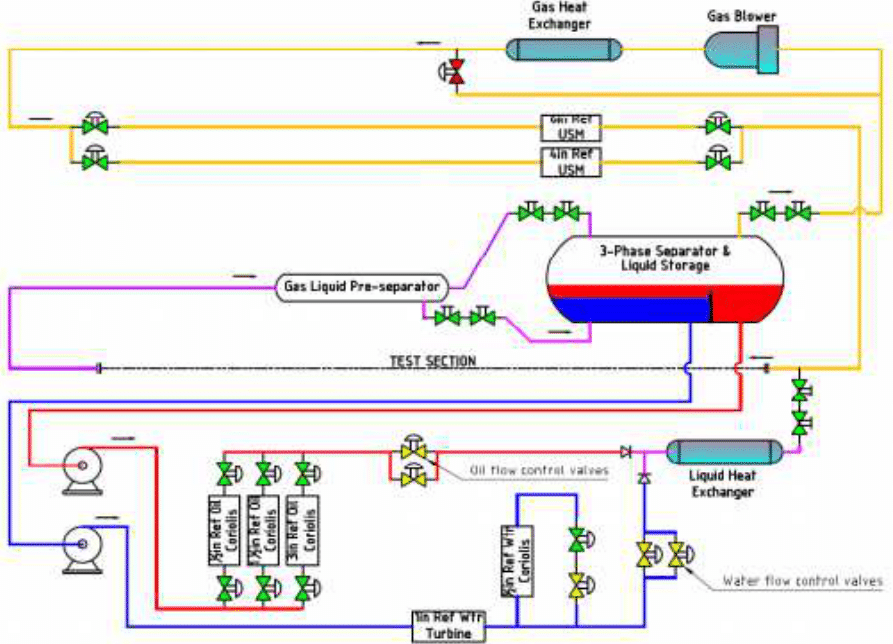
\includegraphics[width=0.9\linewidth]{Figures/test_loop.png}
\centering
\caption{ Test loop schematic \cite{tukimin2016cfd}}
\label{fig:test_loop_rig}
\end{figure}

The CFD model was designed using ANSYS Design Modeller software. The model consists of a Venturi tube designed according to the standards ISO 5167:2003 \cite{iso20035167}, and both a liquid and gas system. The physical experiment was done in a specific test matrix which was included in the numerical simulation model. Finally the coefficient of discharge of the venturi was calculated using equation \ref{eq:2}.  

\begin{equation}
C d=\frac{4 m \sqrt{1-\beta^{4}}}{\pi \varepsilon d^{2} \sqrt{200000 D p_{1} \rho_{1}}}
\label{eq:2}
\end{equation}

\begin{table}[!t]
  \begin{center}
    \leavevmode
    \hangcaption{ \textbf{Calculated $C_{d}$}}   
     \begin{tabular}{rlc}\hline
      Venturi under Test & Average Discharge Coefficient &  Average Discharge Coefficient \\ \hline
       & From experiment &  From CFD post \\ \hline
      Venturi 1 & 0.99366 &  0.984347 \\ \hline
    \end{tabular}
    \label{tab:cd}
  \end{center}
\end{table}
The results obtained in \ref{tab:cd} were found to have a difference of less than $1 \%$.
\par
Tamhankar et al \cite{tamhankar2014experimental} also did a similar experiment using a CFD model in ANSYS Fluent 13.0 utilizing a Realizable k-$\epsilon$ turbulence model which is superior to a Standard k-$\epsilon$ turbulence model and compared the results to those obtained from an experimental setup show in figure \ref{fig:exp}. 

\begin{figure}[ht]
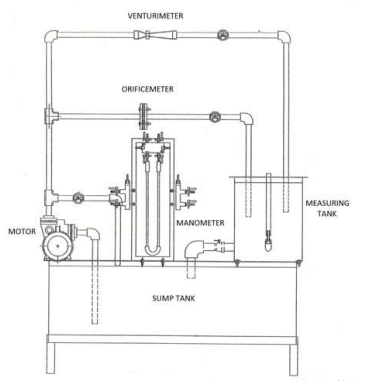
\includegraphics{Figures/exp.png}
\centering
\caption{ Experimental setup \cite{tamhankar2014experimental}}
\label{fig:exp}
\end{figure}

Table \ref{tab:results} shows the results obtained from the experiment
\begin{table}[!t]
    \centering
    \hangcaption{Results}
    \begin{tabular}{|c|c|c|}
        \hline \text { Reading No. } & \text { Experiment } & \text { CFD analysis } \\
        \hline 1 & 0.9724 & 0.9619 \\
        \hline 2 & 0.9592 & 0.9689 \\
        \hline 3 & 0.9779 & 0.9692 \\
        \hline
    \end{tabular}
    \label{tab:results}
\end{table}

The study concluded that difference in values of the coefficient of discharge obtained from the model and the ones obtained experimentally was within $ 5 \%$ .
\subsubsection{Analytical Predictions}
This technique utilizes the Bernoulli's equation to establish an analytical correlation for the coefficient of discharge of the Venturi meter. 

\begin{figure}
    \centering
    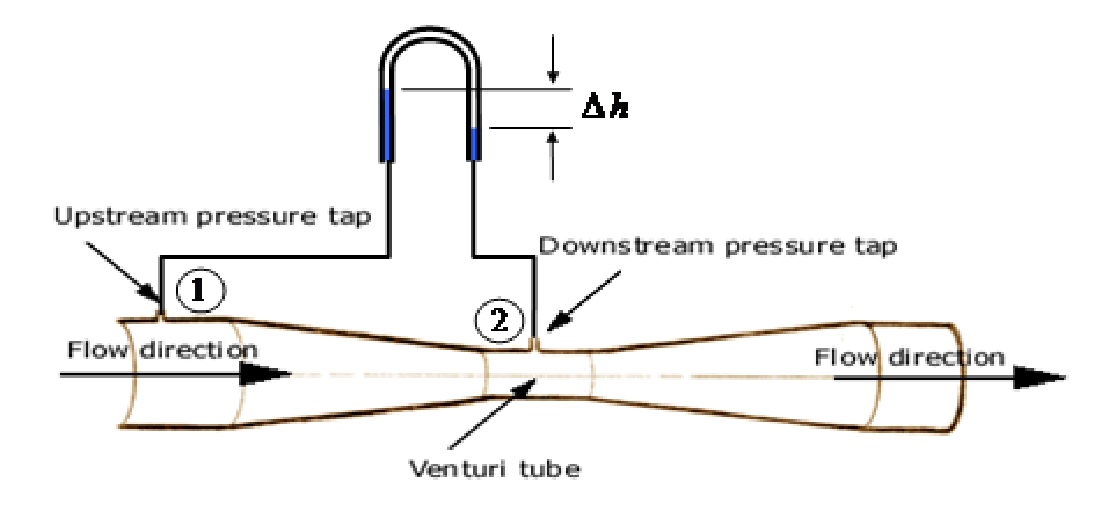
\includegraphics[width=0.6\linewidth]{Figures/venturi.png}
    \caption{Venturi meter}
    \label{fig:venturi}
\end{figure}

Figure \ref{fig:venturi} shows the Venturi meter. Assuming the flow is ideal and applying the Bernoulli's equation before and after the contraction, 

\begin{equation}
\begin{aligned}
&\frac{p_{1}}{\rho g}+\frac{v_{1}^{2}}{2 g}+z_{1}=\frac{p_{2}}{\rho g}+\frac{v_{2}^{2}}{2 g}+z_{2} \\
&\text { But } Z_{1}=Z_{2}, \\
&\frac{\left(p_{1}-p_{2}\right)}{\rho}=\frac{\left(v_{2}^{2}-v_{1}^{2}\right)}{2} \\
&\frac{\left(p_{1}-p_{2}\right)}{\rho}=\frac{v_{2}^{2}}{2}\left(1-\frac{A_{2}^{2}}{A_{1}^{2}}\right) \\
&\frac{\Delta p}{\rho}=\frac{v_{2}^{2}}{2}\left(1-\beta^{4}\right) \\
&v_{2}=\frac{1}{\sqrt{1-\beta^{4}}} \sqrt{\frac{2 \Delta p}{\rho}}
\end{aligned}
\end{equation}

Applying the continuity equation,
\begin{equation}
\begin{aligned}
&Q_{t h}=A_{1} v_{1}=A_{2} v_{2} \\
&Q_{t h}=A_{2} v_{2}=\frac{1}{\sqrt{1-\beta^{4}}} \frac{\pi d^{2}}{4} \sqrt{\frac{2 \Delta p}{\rho}}
\end{aligned}
\end{equation}
The above equation is based on the assumption that the flow is steady, incompressible, inviscid, irrotational, no losses and the velocities $V_{1}$ and  $V_{2}$ are constant across the cross section \cite{arun2015prediction}. 

\begin{equation}
\mathrm{Q}_{\mathrm{act}}=\frac{\mathrm{C}_{\mathrm{d}_{\mathrm{st}} \mathrm{d}}}{\sqrt{1-\beta^{4}}} \frac{\pi \mathrm{d}^{2}}{4} \sqrt{\frac{2 \Delta \mathrm{p}}{\rho}}
\end{equation}
The frictional and viscous losses in laminar flow can be estimated by the Darcy's law
\begin{equation}
\mathrm{H}_{\mathrm{L}}=\frac{(\Delta \mathrm{p})_{\text {viscous }}}{\rho \mathrm{g}}=\mathrm{f} \frac{\mathrm{v}^{2}}{2 \mathrm{~g}} \frac{\mathrm{D}}{\mathrm{D}}
\end{equation}
where 'f' is the friction factor.
\par
Coefficient of discharge equation \ref{eq:cd2} where is for laminar flow 'f' is given by equation \ref{eq:f} . This equation is derived from both the Darcy's law equation and the Bernoulli's equation.
\begin{equation}
f=\frac{64}{R_{e d}}
\label{eq:f}
\end{equation}


\begin{equation}
C_{\mathrm{d}}=0.995 \sqrt{\frac{1}{(1+3 f)}}
\label{eq:cd2}
\end{equation}

\par
Arun et al \cite{arun2015prediction} did  a comparision of the $C_{d}$ obtained by this method and the obtained from CFD.
The study concluded that the results from the two methods had an uncertainity of $0.9\%$.
\subsection{Related Works}
Discharge collection process and techniques have existed over a long time and finds application in various sectors. 
\subsubsection{Pressure Control }
To solve the problem of sludge deposits accumulating in storage tanks, Liu et al,\cite{liu2018research} proposed a new set of an automatic adjusting underwater sludge discharge collector and regulator  as shown in figure \ref{fig:sludge1} . 
\begin{figure}[ht]
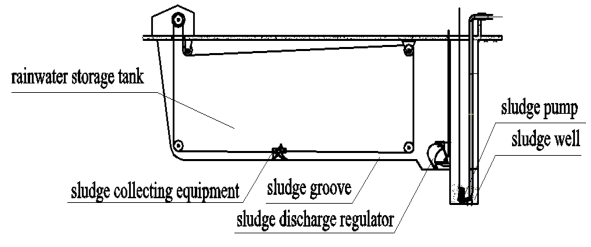
\includegraphics[width=0.9\linewidth]{Figures/sludge1.png}
\centering
\caption{ The Principle of Underwater Sludge Discharge and Collection System \cite{liu2018research}}
\label{fig:sludge1}
\end{figure}
\begin{figure}[ht]
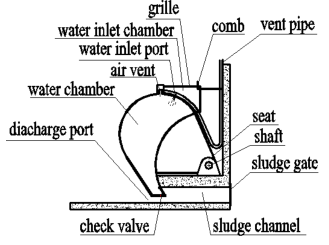
\includegraphics[width=0.7\linewidth]{Figures/sludge 2.png}
\centering
\caption{ The Structure and Principle of the Sludge Discharge Regulator \cite{liu2018research}}
\label{fig:sludge 2}
\end{figure}
The regular employs the use of a check valve to adjust the water pressure inside the water chamber as shown in figure \ref{fig:sludge 2}. Blockage in the discharge port reduces the flow in the sludge channel thus lowering the pressure of the sludge channel as to that of the water chamber. This causes a drop a water level drop in the water chamber reducing the weight of the regulator. A reduction in the regulator weight, enlarges the discharge port and thus the blocked sludge is released and collected.
\subsubsection{Electromagnetic activation}
Angelo et al \cite{odetti2019design} implemented this technique in the design and testing of an Modular Automatic Water Sampler (MAWS). They designed MAWS and mount them on Unmanned Marine Vehicles (UMV) with the aim of collecting water samples for scientific campaigns in front of polar tidewater glaciers. Their main design considerations was the response time of the stopper since MAWS were operated under water and at the risk of damage by glaciers. The actuation unit of the sampler is shown in figure \ref{fig:stopper} . 

\begin{figure}
    \centering
    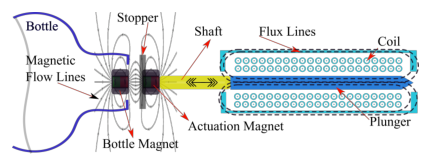
\includegraphics{Figures/stopper.png}
    \caption{Sampler actuation mechanism \cite{odetti2019design}}
    \label{fig:stopper}
\end{figure}
When the coil in the solenoid is crossed by a currrent a strong magnetic field is generated that attracts the ferromagnetic plunger connected to the sealing stopper and opens the bottle allowing water flowing into the bottle's neck. As the current stops the two permanent magnets attract each other and the stopper seals the bottle \cite{odetti2019design}.

\subsection{Summary}

Every fluid flow experiment done on the Synthetic Hydro-Experimental machine involves collecting the discharge and its properties. The most common experiment is the determination of the coefficient of discharge  of the Venturi and the Orifice. In this literature, other techniques such as CFD and analytical methods have been found to be effective in this experiment. Both techniques have been proven to produce results with a difference of less than $1\%$  from the experimental results. Such results can also be obtained by the fluids rig currently used in JKUAT by automating the discharge collection unit. The literature has also covered techniques that also be used to achieve this such as the application of pneumatics and electromagnets.

\subsection{Gap Analysis}

\begin{enumerate}
    \item 
\end{enumerate}


